\documentclass[12pt]{article}
\DeclareMathSizes{12}{13}{10}{9}
\usepackage[utf8]{inputenc}
\usepackage[margin=1.5cm]{geometry}
\usepackage{amsmath}
\usepackage{amssymb}
\usepackage{amsthm} % allows example and proof environment to be defined/used
\usepackage{cancel}
\usepackage{graphicx}

\newtheorem*{esempio}{Esempio}

\begin{document}
\section*{Lezione 3}
\subsection*{Struttura del sistema floating-point}
In questa lezione studieremo la struttura del sistema floating-point, ovvero dell'insieme dei reali-macchina e dei reali rappresentabili per arrotondamento tramite i reali-macchina.\\
Tratteremo un sistema astratto in base $b$ generica (come fatto finora, con esempi in base 10), per poi discutere un modellino semplificato dello standard a 64 bit (base 2), utilizzato in Matlab e in tutti i principali linguaggi di calcolo.\\
Ricordiamo che i reali-macchina in base $b$ a $t$ cifre di mantissa e con range di esponenti $[L,U] \subset \mathbb{Z}$ sono definiti da
\[ \mathbb{F}(b, t, L, U) = \{ \mu \in \mathbb{Q} : \mu = sign(\mu)\cdot (0,\mu_1 \mu_2 \dotsc \mu_t) \cdot b^p \,,\, \mu_j \in \{ 0, 1, \dotsc, b-1 \} \,,\, \mu_1 \ne 0 \,,\, p \in [L,U] \subset \mathbb{Z} \} \]
dove $\mu_j$, $j = 1, \dotsc, t$ sono le cifre della mantissa e $p$ l'esponente intero della potenza della base che sposta la virgola dove $L<0$ e $U>0$, quindi $p$ appartiene all'intervallo di interi $L, L+1, \dotsc, -1, 0, 1, \dotsc, U-1, U$.\\
Risponderemo ad alcune domande di base:
\begin{itemize}
    \item quanti sono i reali-macchina?
    \item quali reali sono approssimabili per arrotondamento con i reali-macchina?
    \item come sono distribuiti sull'asse reale i reali-macchina?
\end{itemize}
In modo molto schematico, sintetizziamo con un disegno \newline
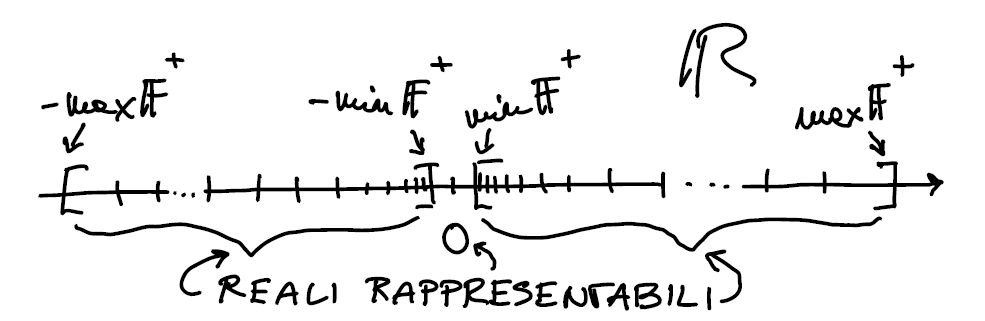
\includegraphics[width=\linewidth]{img2}
In questo schemino grafico i reali-macchina corrispondono all'insieme \underline{finito} di tacche sull'asse reale e a parte lo 0 che è un reale-macchina (con una rappresentazione speciale visto che la mantissa nulla non è ammessa) \underline{stanno nell'unione di due intervalli simmetrici}. Infatti, detti $\mathbb{F}^+$ i reali-macchina $>0$ e $\mathbb{F}^-$ quelli $<0$, abbiamo che $\mathbb{F}^- = - \mathbb{F}^+$ (cioè si cambia segno a tutti i positivi, $\mathbb{F}^+$ e $\mathbb{F}^-$ sono simmetrici rispetto a 0) 
\[ \mathbb{F}^+ \subset [\,\min \mathbb{F}^+, \max \mathbb{F}^+\,] \]
\[ \mathbb{F}^- \subset [\,- \max \mathbb{F}^+, - \min \mathbb{F}^+\,] \]
Questi \underline{due intervalli} nel continuo sono proprio i \underline{reali approssimabili} tramite i reali-macchina per arrotondamento a $t$ cifre della mantissa, con un errore relativo $\le \varepsilon_M = \frac{b^{1-t}}{2}$ (la precisione di macchina). Invece i reali che in modulo sono $> \max \mathbb{f}^+$ e quelli che in modulo solo $< \min \mathbb{f}^+$, sono "troppo grandi" o "troppo piccoli" per essere approssimati e costituiscono quello che si chiama l'OVERFLOW e l'UNDERFLOW nel sistema floating-point.\newline
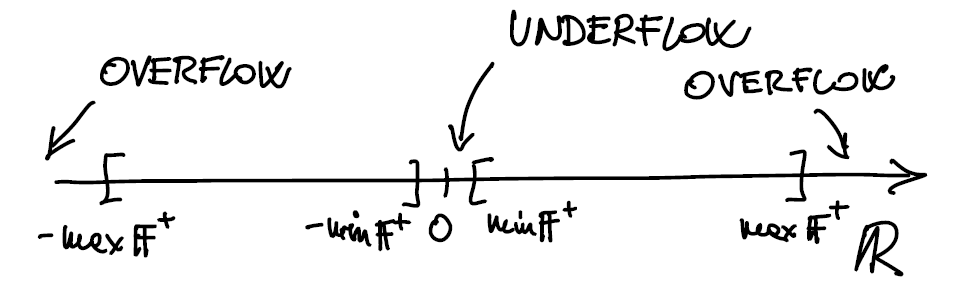
\includegraphics[width=\linewidth]{img3}
L'UNDERFLOW è un intorno di 0, l'OVERFLOW un intorno di $\infty$.\\
Il problema è che l'esponente $p$ di tali numeri è fuori dal range di esponenti ammissibili, ovvero $[L,U] \subset \mathbb{Z}$ (cioè $p < L$ (underflow) oppure $p > U$ (overflow)).\\
La comparsa di numeri in overflow/underflow durante un processo di calcolo altera il processo stesso facendogli tendenzialmente perdere di significato. \\
Nei vecchi linguaggi di programmazione (ad esempio il Fortran) la comparsa di overflow determinava addirittura l'arresto del processo di calcolo con un messaggio di errore. In Matlab invece (e in altri linguaggi) un numero in overflow, generato ad esempio dal prodotto di reali-macchina molto grandi in modulo, viene indicato con simbolo "\texttt{Inf}" (infinito) ed entra nel processo di calcolo alterandolo, generando altri "\texttt{Inf}" o forme indeterminate (ad es.$\frac{\texttt{Inf}}{\texttt{Inf}}$) che vengono indicate col simbolo "\texttt{NaN}" (Not a Number).\\
Per questo negli algoritmi numerici è importante cercare di prevenire overflow/underflow. \\
A questo punto conviene calcolare $\min \mathbb{F}^+$ e $\max \mathbb{F}^+$, modo da quantificare gli estremi degli intervalli di rappresentazione visto che un reale-macchina ha la struttura 
\[\mu = \text{segno} \cdot \text{mantissa} \cdot b^p\]
Il minimo positivo si otterrà moltiplicando la minima mantissa per la potenza della base con il minimo esponente
\[ \text{\underline{mantissa minima}} = (0,10 \dotsc 0)_b = 1 \cdot b^{-1}\]
\[ \text{\underline{esponente minimo}} = L\]
quindi
\begin{table}[h!]
    \centering
    \begin{tabular}{|c|}
    \hline
        $\min \mathbb{F}^+ = b^{L-1}$ \\
    \hline
    \end{tabular}
\end{table}
Invece il massimo positivo si otterrà moltiplicando la mantissa massima per la potenza della base col massimo esponente
\[ \text{\underline{mantissa massima}} = (0,\underbrace{b-1} \underbrace{b-1} \dotsc \underbrace{b-1})_b\]
cioè tutte le $t$ cifre sono uguali alla cifra massima che è $b-1$
\begin{esempio}
$(0,99 \dotsc 9)_{10}$ in base 10
\end{esempio}
Calcoliamo usando la somma geometrica di ragione $b^{-1}$
\[\begin{split}
    \text{\underline{mantissa max}} & = \sum_{j=1}^t\,(b-1)\,b^{-1} \\
    & = (b-1)\,\sum_{j=1}^t\,b^{-1} \\
    & = (b-1)\,\biggl(\sum_{j=0}^t\,b^{-1} - 1\biggr) \\
    & = (b-1)\,\biggl(\frac{1 - b^{-(t+1)}}{1 - \frac{1}{b}} - 1\biggr) \\
    & = (b-1)\,\biggl(\frac{b - b^{-t}}{b - 1} - 1\biggr) \\
    & = 1 - b^{-t} \\
\end{split}\]
Ora \[ \text{\underline{esponente massimo}} = U\] quindi
\begin{table}[h!]
    \centering
    \begin{tabular}{|c|}
    \hline
        $\max \mathbb{F}^+ = (1 - b^{-t})\,b^U$ \\
    \hline
    \end{tabular}
\end{table}
\begin{esempio} \end{esempio}
in base 10 con 16 cifre di mantissa ed esponenti minimo $L = - 307$ e massimo $U = + 308$ (modello che come vedremo corrisponde in sostanza all'interfaccia del Matlab, ben sapendo però che la base interna del calcolatore è 2 e non 10)
\[ \min \mathbb{F}^+ = 10^{- 1 - 307} = 10^{- 308} \]
\[ \max \mathbb{F}^+ = (1 - 10^{-16})\cdot 10^{308} \approx 10^{308}\]
\newline \newline
I reali rappresentabili tramite reali-macchina in Matlab sono quindi intervalli estremamente ampi, con un estremo "grandissimo" e un estremo "piccolissimo" (in modulo, considerando anche l'intervallo dei negativi). \\
È importante però ricordare ancora una volta che la rappresentazione avviene per arrotondamento della mantissa e che gli \underline{unici} numeri effettivamente memorizzabili nel calcolatore sono i \underline{reali-macchina}, un \underline{insieme finito}.\\
Ma qual è la \underline{cardinalità} (numero di elementi) di $\mathbb{F}$? Il calcolo è facile, osservando che basta contare gli elementi di $\mathbb{F}^+$ e raddoppiare, tenendo poi conto dello 0 che ha una rappresentazione speciale
\[\begin{split}
    \text{card}(\mathbb{F}^+) & = \text{numero possibili mantisse} \,\cdot\, \text{numero possibili esponenti} \\
    & = (b-1)\cdot \underbrace{b \cdot \dotsc \cdot b}_{t - 1 \,\text{fattori}} \cdot \, (U - L + 1) \\
    & = (b-1)\cdot b^{t - 1} \cdot \, (U - L + 1) \\
\end{split}\]
In questo conto si osservi che per la prima cifra di mantissa ci sono $b - 1$ scelte (non può essere 0), mentre ci sono $b$ scelte per tutte le altre cifre (ad es. in base 10 la prima cifra può essere $1, 2, \dotsc , 9$ cioè 10 possibili cifre). \\
Il numero di elementi dell'intervallo di interi $[L,U]$ è $U-L+1$. Alla fine si ottiene
\[ \text{card}(\mathbb{F}) = 1 + 2 \cdot (b-1)\cdot b^{t - 1} \cdot \, (U - L + 1) \]
Nel modello simil-Matlab visto prima con $b = 10$, $t = 16$, $L = -307$, $U = +308$ si ottiene \[ \text{card}(\mathbb{F}) = 1 + 2 \cdot 9\cdot 10^{15} \cdot \, 616 \]
che è un numero dell'ordine di $10^{19}$.\\
Da dove vengono i parametri che abbiamo usato per il modello simil-Matlab? Dal fatto che il Matlab usa uno standard di rappresentazione per i reali-macchina (lo standard IEEE) in cui ad una variabile reale è dedicata una sequenza di 64 bit (8 byte), in cui 1 bit è riservato al segno, 52 bit alla mantissa e 11 bit all'esponente. \\
Senza entrare in dettaglio nello standard di rappresentazione facciamo un semplice modello:\newline
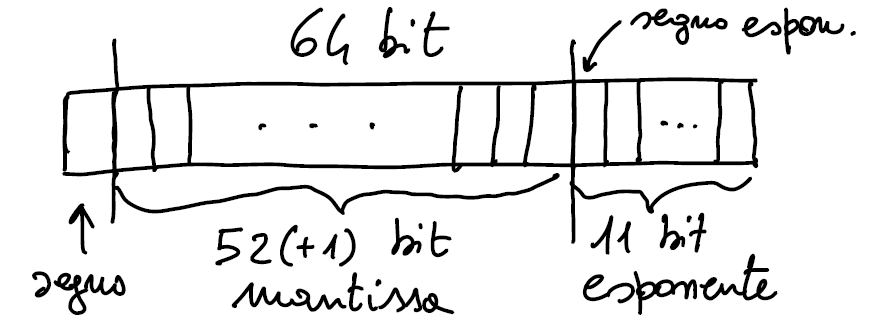
\includegraphics[width=\linewidth]{img4}
In ciascuna delle caselline (bit) si può scrivere 0 oppure 1 (per il segno uno dei due rappresenta "+" e l'altro "-"). Per quanto riguarda la mantissa i bit sono 52 ma è come se fossero 53, perchè la prima cifra di mantissa deve essere non nulla e quindi per forza 1 (ovvero il processore tratta i numeri come se avessero mantissa $0,1 d_2 \dotsc d_{53}$ con $d_j \in \{0,1\},\, 2 \le j \le 53$) quindi la \underline{precisione di macchina} è
\[ \varepsilon_M = \frac{2^{1-53}}{2} = 2^{-53} \approx 10^{-16}\]
Per quanto riguarda il range di esponenti, in questo modello semplificato degli 11 bit a disposizione ne teniamo uno per il segno. Quindi $\max \, \lvert \, p \, \rvert$ si ottiene con la sequenza
\[ (\underbrace{11\dotsc1}_{\text{10 cifre}})_2 \]
ovvero
\[ \max \, \lvert \, p \, \rvert = \sum_{j=0}^9 2^j = \frac{2^{10} - 1}{2 - 1} = 1023 \]
Ricordando le proprietà della somma geometrica (qui con ragione 2) viste nella lezione 1, allora \[ U = +1023 \,,\, L = -1023 \] e
\[ \max \, \mathbb{F}^+ \, \approx 2^{1023} \approx 10^{308}\]
\[ \min \, \mathbb{F}^+ \, = 2^{-1024} \approx 10^{-308}\]
(in realtà la codifica dell'esponente usa una tecnica un po' più sofisticata ma la sostanza cambia poco) \\
Alla fine possiamo dire che in Matlab (e molti altri linguaggi) i reali-macchina sono sequenze a 64 bit (la cosiddetta precisione doppia) corrispondenti sostanzialmente a
\[ \mathbb{F}(2, 53, -1023, +1023) \]
Siccome l'interfaccia dei linguaggi con l'utente è in base 10 (con conversione automatica dell'input/output) per quanto visto sopra possiamo dire che lavorando in Matlab è essenzialmente (ma non esattamente) come se utilizzassimo
\[ \mathbb{F}(10, 16, -307, +308) \]
nel senso che l'ordine di grandezza dei parametri chiave $\varepsilon_M, \max \mathbb{F}^+, \min \mathbb{F}^+$ è corretto (ma scopriremo che talvolta bisogna tener presente che la base "vera" è 2). \\
Finora abbiamo risposto a due delle tre domande iniziali sulla struttura del sistema floating-point, resta da analizzare come sono distribuiti i reali-macchina. \\
Il concetto chiave è che \underline{non} sono distribuiti \underline{uniformemente}, ma bensì "\underline{a densità variabile}", i reali-macchina "piccoli" sono vicini, i reali-macchina "grandi" sono distanti tra di loro, la densità cresce andando verso $\pm \min \mathbb{F}^+$ e decresce andando verso $\pm \max \mathbb{F}^+$. \\
Questo si può capire bene calcolando la distanza tra reali-macchina consecutivi (con lo stesso esponente $p$).\\
Graficamente (ad es. in $\mathbb{F}^+$) \newline
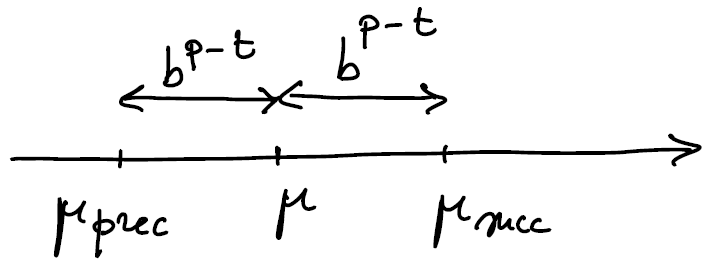
\includegraphics[width=\linewidth]{img5}
Infatti due reali-macchina consecutivi differiscono di 1 nella $t$-esima cifra di mantissa, ovvero
\[ \text{mantissa}(\mu_{\text{succ}})\,-\,\text{mantissa}(\mu) = 1 \cdot b^{-t}\] e 
\[ \mu_{\text{succ}}\,-\,\mu = b^{-t} \cdot b^p = b^{p-t} \]
La distanza (assoluta) è quindi variabile con $p$, cioè con l'ordine di grandezza del numero in base $b$. \\
Questa distanza varia (di un fattore $b$) quando si passa per una potenza della base.
\begin{esempio}
$b = 10$ e $t = 2$ (due cifre di mantissa) \newline
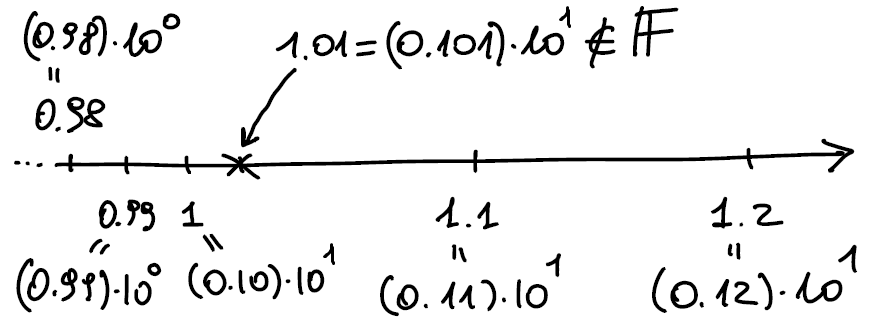
\includegraphics[width=\linewidth]{img6}
\end{esempio}
La domanda è: chi è il reale-macchina successivo ad 1? Pensando a 2 cifre decimali, verrebbe da rispondere 1,01 ma \underline{non} è così, perchè $1,01 = (0,101)\cdot 10^1$ ha 3 cifre di mantissa e in questo esempio $t=2$.\\
Invece il reale-macchina successivo ad 1 è $(0,11)\cdot 10^1 = 1,1$ passando per $1 = 10^0$ la distanza è cresciuta di un fattore 10, da $10^{-2}$ a $10^{-1}$.\\
Pensando invece a quali reali sono approssimati da 0,99, 1 e 1,1 abbiamo graficamente \newline
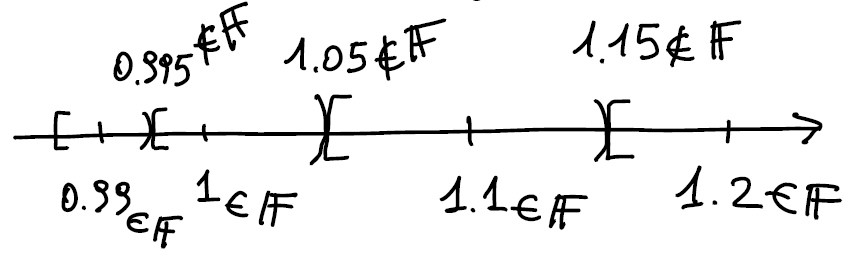
\includegraphics[width=\linewidth]{img7}
Vediamo che ogni reale-macchina è il centro di un intorno di approssimazione a $t$ cifre di mantissa (qui $t=2$): questi intorni sono generalmente simmetrici e di raggio $\frac{b^{p-t}}{2}$ \newline
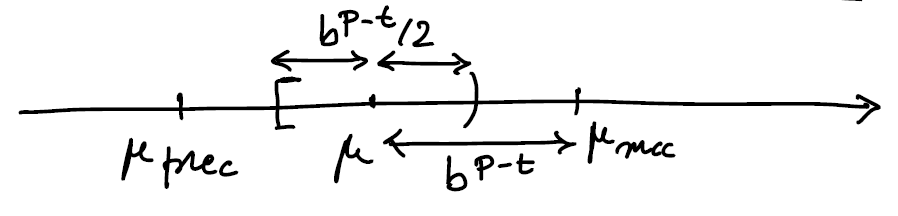
\includegraphics[width=\linewidth]{img8}
tranne per $\mu = b^k$, nel qual caso l'intorno è asimmetrico e l'intorno destro (in $\mathbb{F}^+$) si allunga di un fattore $b$.\\
Tutti i reali di questi intorni vengono approssimati dal reale-macchina centro dell'intorno per arrotondamento a $t$ cifre di mantissa, con un errore assoluto $\le \frac{b^{p-t}}{2} =$ raggio. Ma se andiamo a stimare l'\underline{errore relativo}, sappiamo dalla lezione 2 che questo non può superare la precisione di macchina \[ \varepsilon_M = \frac{b^{1-t}}{2} \]
che è \underline{indipendente da $p$}.\\
L'unione di tutti gli intorni di approssimazione per arrotondamento copre gli intervalli dei reali rappresentabili, ovvero
\[ [- \max \mathbb{F}^+ , - \min \mathbb{F}^+] \cup [\min \mathbb{F}^+ , \max \mathbb{F}^+]\]
Come descritto in modo un po' ingenuo da questo disegno (per $\mathbb{F}^+$) \newline
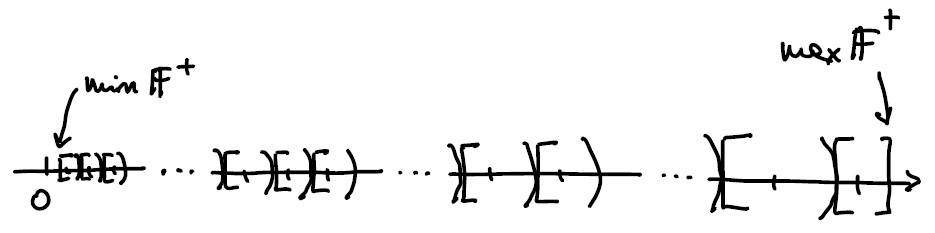
\includegraphics[width=\linewidth]{img9}
Concludiamo questa lezione con due esempi semplici in base 10:
\begin{esempio} \end{esempio}
Disegnare $\mathbb{F}(10, 1, -1, 1)$ \\
Abbiamo una sola cifra di mantissa (il minimo possibile) ed esponenti $p = -1, 0, 1$.\\
Disegniamo $\mathbb{F}^+$ (scrivendo per semplicità i reali-macchina in notazione standard) \newline
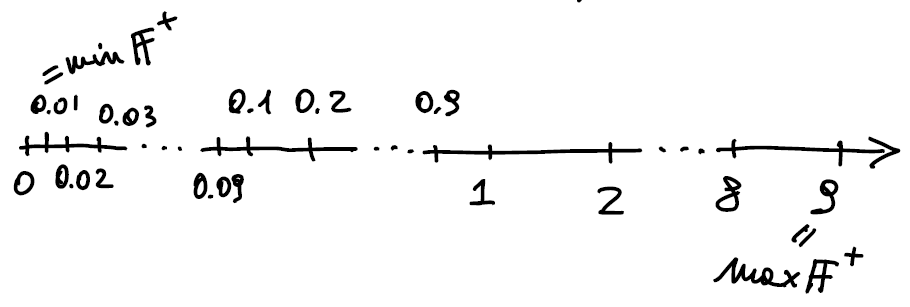
\includegraphics[width=\linewidth]{img10}
Vediamo che si parte dall'ordine di grandezza dei centesimi con 
\[ \min \mathbb{F}^+ = 0,1 \cdot 10^{-1} = 0,01 \]
(tra i centesimi non ci sono reali-macchina perchè c'è una sola cifra di mantissa), si passa ai decimi, poi alle unità sempre senza reali-macchina intermedi, fino a
\[ \max \mathbb{F}^+ = 0,9 \cdot 10^1 = 9 \]
La precisione di macchina è 
\[ \varepsilon_M = \frac{10^{1-t}}{2} = \frac{10^{1-1}}{2} = \frac{1}{2} = 50\% \]
Si tratta di un sistema floating-point molto "povero", perchè c'è una sola cifra di mantissa e un'estensione molto limitata dal piccolo range di esponenti.

\begin{esempio} \end{esempio}
Disegnare $\mathbb{F}(10, 2, -2, 2)$ \textbf{PER ESERCIZIO} (converrà fare degli opportuni "zoom" sui vari ordini di grandezza). Il sistema è più "ricco" del precedente, infatti abbiamo
\[ \min \mathbb{F}^+ = b^{L-1} = 10^{-3} \]
\[\begin{split}
    \max \mathbb{F}^+ & = (1 - b^{-t}) \cdot b^U \\
    & = (1 - 10^{-2}) \cdot 10^2 = 99
\end{split}\]
\[ \varepsilon_M = \frac{b^{1-t}}{2} = \frac{10^{-1}}{2} = 5\% \]
Si parte dai millesimi, ma fra questi ci sono i decimillesimi perché abbiamo 2 cifre di mantissa, poi ai centesimi con i millesimi, i decimi con i centesimi, le unità con i decimi e infine le decine con le unità.
\newline \newline
Questo dovrebbe far capire quanto ricca è la struttura del sistema floating-point a 64 bit (\underline{precisione doppia}). \\
È il caso di ricordare che esistono altri standard, la precisione \underline{singola} (a 32 bit) con $\varepsilon_M \approx 10^{-8}$ e la precisione \underline{quadrupla} (a 128 bit) con $\varepsilon_M \approx 10^{-32}$.\\
Quale sia la precisione di default dipende dal linguaggio, alcuni permettono di scegliere tra singola, doppia e quadrupla. \\
Queste precisioni corrispondono ad operazioni aritmetiche implementate a livello hardware (circuiti) nel processore, quindi estremamente veloci. \\
In alcuni linguaggi è possibile aumentare la precisione (cioè aumentare il numero di cifre di mantissa), ma allora le operazioni aritmetiche sono implementate a livello software (c’è un programma che calcola somma, moltiplicazione e divisione, non un’unità hardware), quindi il costo delle operazioni cresce e cresce ovviamente l’occupazione di memoria, soprattutto elaborando masse di dati. \\
Questo è il motivo per cui si è fatto un compromesso e lo standard attuale è la precisione doppia con $\varepsilon_M = 2^{-53} \approx 10^{-16}$, un massimo errore relativo di arrotondamento che è di solito molto più piccolo degli errori di misura sperimentale dei dati nelle applicazioni.\\
Ciononostante, vedremo che la propagazione degli errori in algoritmi instabili può far perdere anche tutta questa precisione nel processo di calcolo. \\
Questo conduce in modo naturale allo studio della STABILITÀ degli algoritmi numerici, che cominceremo già nella prossima lezione sulle operazioni aritmetiche con numeri approssimati.
\end{document}